\chapter{Implementation methodology}
As stated before we want to evaluate the performance of CNN's to reconstruct images from compressed measurements. In this chapter we will describe the tools and software frameworks used in order to build the set-up for our experiments. First,  we introduce some of the most widely used libraries to build and train neural networks and the specific software tools for this thesis. Second, we briefly describe Graphics Processing Units (GPU's) and give reasons why they are an important tool when working with deep learning. Third, we will describe the datasets for training the networks and briefly justify its utilization. Then, we explain how the data is pre and post-processed. This is important since it allows to efficiently use the hardware resources and makes the training process numerically stable. Finally, we propose CNN architectures for the reconstruction process.   

\section{Theano}
Theano is a library written in python that permits to define, optimize and compute mathematical expressions that deal with high-dimensional arrays in an efficient way. It is widely used among the deep learning community because it is optmized to make use of GPU routines that make training faster, efficient symbolic differentiation, stability optimizations and therefore making it realiable since it is constantly tested and debugged \cite{2016arXiv160502688short}. Nevertheless, Theano is not intended to be used only for neural natwork applications. Therefore, it is necessary to write routines or API's that specially handle the difficulties encountered for deep learning. Such applications are normally an extra abstraction layer that sits on top of Theano's implementation and specially allow to build and train neural networks. Examples publically avaible are Lasagne \cite{sander_dieleman_2015_27878}, Blocks \cite{van2015blocks} and Keras \cite{chollet2015keras}. \
Other common frameworks in deep learning are Google's Tensorflow \cite{tensorflow2015-whitepaper} that is written in C++, Torch \cite{torch} written in Lua and Caffe \cite{jia2014caffe} also written in C++. Most of them offer the same characteristics and mostly differ in the language they are written in, speed and target application, for example Caffe is not suitable for audio and text applciations.           
\subsection{Sdeepy}
Due to the fact that the previously mentioned implementations are constantly updated and changing, Sony decided to develop its own library to develop their projects. Sdeepy is an in-house Sony's deep learning library implementation that makes use of Theano and incorporates routines commonly used as building-blocks for training and testing neural networks. It has the advantage that many new features can be added at any time they become available while maintaining the stability. Furthermore, it is easier to adapt and modify according to one's needs. Because of all that, we will use Sdeepy for this thesis but all implementations might be easily translated into any available framework.
\section{Graphics Procesing Unit (GPU)}
\begin{figure}[tb] 
\centering 
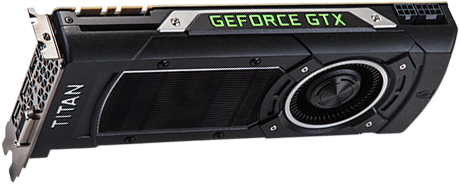
\includegraphics[scale=0.7]{GPU1.png} 
\caption[GPU for deep learning]{NVIDIA graphics card GeForce GTX Titan X used in our experiments.}
\label{fig:GPUim1} 
\end{figure}
A Graphics Processing Unit (GPU) is a chip architecture mainly designed for imaging and gaming. It differs from general-purpose CPU's in that they can handle larger amounts of data efficiently and faster in a parallel way, making them much more suitable for deep learning applications. It has extended its usage into machine learning area because companies like NVIDIA have develop GPU's specially optimized for neural networks. Not only that, but they have also written routines (NVIDIA Deep Learning SDK) that improve and speed up common operations like convolutions, better memory management and friendlier API's for easy learning. By distributing the workload of the training process the convergence happens much faster than by using conventional CPU's. See Figure \ref{fig:GPUim1} and Table \ref{tab:GPU1} .

\begin{table}[tb]
\caption[Technical speficications of GeForce GTX Titan]{Technical details of the GPU}
\label{tab:GPU1}
\centering
\begin{tabular}{l*{6}{c}r}
\hline
Architecture   & Maxwell\\
CUDA cores   & 3072\\
Base clock speed   & 1000MHz\\
Boost clock speed   & 1075MHz\\
Memory type   & GDDR5\\
Memory    & 12GB\\
Memory Bandwidth    & 7Gbps\\
Memory interface width    & 384-bit\\
\bottomrule 
\end{tabular}  
\end{table}

\section{Datasets}
It is also important to mention that along with better hardware and more ingenious algorithms, deep learning has achieved major success because in recent years more and more data is becoming available through the internet. For most of machine learning methods data is the most important asset to obtain successful results. In fact, choosing the right dataset is the first step in the deep learning work-flow cycle and it is, in general, more important than the chosen learning algorithm itself. \
Since our goal is to reconstruct images, we make use of three different image datasets: BioID \cite{frischholz2003bioid}, Label faces in the wild (LFW) \cite{LFWTech} and LabelMe \cite{russell2008labelme}. The first two datasets served as an initial baseline for measuring the plausibility of our approach and the last one allows for a more robust justification as explained later. All of the datasets are known in the community for being applied to different computer vision tasks like face detection, emotion recognition and image classification. Here, we propose its usage for image reconstruction from compressed samples. 
\begin{table}[tb]
\caption[Datasets for training and testing]{Original features of each dataset.}
\label{tab:datasets1}
\centering
\begin{tabular}{l*{6}{c}r}
Dataset name              & Number of images & training & testing &  Original image size& Grayscale \\
\hline
BioID   & 1521 & 1371 & 150 & 384x286 & Yes\\
LFW     & 13233 & 11933 & 1300 & 250x250 & No\\
LabelMe & 50000 & 40000 & 10000 & 256x256 & No\\
\bottomrule 
\end{tabular}  
\end{table}

All datasets differ in terms of image size, color model (RGB or Grayscale) and file format (jpg, png, bmp, etc.). In order to facilitate implementation, all datasets had to be transformed into a more generic form that could meet our constraints. Namely, it is more convenient to work with grayscale images and once promising results are obtained, it can be easily extended to RGB images or even video. For that reason, LFW and LabelMe datasets were converted into grayscale images using rgb2gray MATLAB function. Furtheremore, having an image size that was divisible by 16 was an initial requirement and so each image was resized to $256x256$ using imresize. The actual data being used is described in table \ref{tab:datasets2}.   
\begin{table}[tb]
\caption[Transformed datasets for training and testing]{Transformed features of each dataset.}
\label{tab:datasets2}
\centering
\begin{tabular}{l*{6}{c}r}
Dataset name              & Number of images & training & validation &  Original image size& Grayscale \\
\hline
BioID   & 1521 & 1371 & 150 & 256x256 & Yes\\
LFW     & 13233 & 11933 & 1300 & 256x256 & Yes\\
LabelMe & 50000 & 40000 & 10000 & 256x256 & Yes\\
\bottomrule 
\end{tabular}  
\end{table}

Finally, in order to evaluate the performance of our trained network we introduce a set of 18 images. The images, we believe, are the most popular ones in the image processing community and serve as a baseline for many reconstruction algorithms and image processing tasks. They also help compare our results against the ones reported by other researchers. The evaluation set is shown in figure \ref{fig:EVALim1}
\begin{figure}[tb] 
\centering 
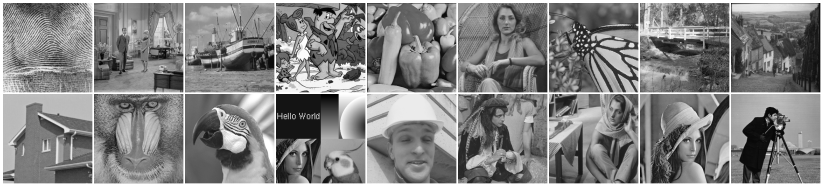
\includegraphics[scale=0.7]{EVAL1.png} 
\caption[Evaluation images]{From Top Left to Bottom Right: 'fingerprint', 'couple', 'boats', 'flintstones', 'peppers', 'woman', 'butterfly', 'bridge', 'houses', 'house', 'mandril', 'parrot', 'montage', 'foreman', 'man', 'barbara', 'lena', 'cameraman'}
\label{fig:EVALim1} 
\end{figure}

\subsection{Training set}
Consist of the largest set of images and is the one used for learning the optimum values of $\omega$ parameters during training. Because one can argue that fitting $\omega$ values to a particular dataset may lead to overfitting and therefore the network could perform poorly with unseen data we have to test our model with different data. Column training in table \ref{tab:datasets2} refers to the number of training images for each dataset.

\subsection{Validation set}
Is a smaller part of the dataset that is not used for training. Since, the training images also come from the same distribution, correlations about the performance in in this data help decide whether the CNN is overfitting the data or how good the generalization is. Column validation in table \ref{tab:datasets2}  gives the number of validation images for each dataset. 

\subsection{Testing set}
This a set of images we introduce in order to further test out CNN. It's not used or linked in anyway to the training process and serves more as a proof of the CNN's performance. We divide the set from the tradition of using certain famous images for showing results of an images processing algorithm.

\section{Preprocessing of the images for supervised learning} \label{sec:prepro}
Even though grayscale images can be easily interpreted as a 2D matrix, CNN's expect as an input a 3D tensor, chapter 2.2.2, complying with the convention depth, height and width. Consequently, extra preprocessing is carried out to generate the data set that is used as the final input of the network for training. Moreover, we make use of a technique called Block Compressed Sensing (BCS). BCS allows to divide the image into small blocks of size $B \times B$ and then compress them by using the same sensing matrix $\Phi$. It has the main advantage of having a small sensing matrix that can be easily extended to process high-dimensional images and making the overall process faster \cite{gan2007block, fowler2012block}. Another important parameter is the compression rate $C$. That is, how much information we would like to sense. For most of our experiments the we choose $C=16$ (we also show results with different $C$ values).           \
\\\\
To demonstrate the process, consider an image randomly taken from one of the datasets. It has a size of $M \times N$. First, it is converted into  blocks of size $B \times B$, where $B=16$, by using MALAB command im2col. Second, each block is multiplied with the sensing matrix $\Phi$ to obtain the measurements. That is, blocks of size $16 \times 16  = 256$ samples, with $C=16$ we only take $ \frac{256}{16}=16$ measurements per block. There are $16 \times 16 $ blocks, thus $16 \times 16 \times 16$ measurements in total for an image of size $M=256 \times N=256$. A pictorial representation of the process can be seen in Figure \ref{fig:PREPROim1}. $\Phi$ is the sensing matrix of size $C \times  ( pixels \enspace per \enspace block) = C \times B^2$ and each block has $B \times B pixels$. Then, the blocks are vectorized so that they have a shape $B^2 \times 1$ and consequently multiplied with $\Phi ( C \times B^2 )$ yielding a final measurement shape $C \times 1 $. Finally, after preprocessing each image individually, the data used for training and testing is a 4D tensor and each dimension is interpreted as follows: $(Number \enspace of \enspace images, \enspace size \enspace of \enspace C ,\enspace size \enspace of \enspace \frac{M}{B} , \enspace size \enspace of \enspace \frac{N}{B}$.  
\begin{figure}[tb] 
\centering 
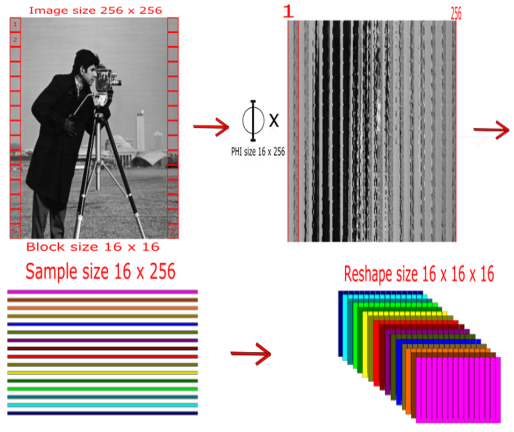
\includegraphics[scale=0.38]{PREPRO1.png} 
\caption[Preprocessing of images]{Example of image preprocessing  with $B=16$, $M=16$ and $N=256$.}
\label{fig:PREPROim1} 
\end{figure}

\section{Preprocessing of the images for unsupervised learning} \label{sec:preproun}
The preprocessing of the data for unsupervised learning is very similar to the approach explained in section \ref{sec:prepro}. The main difference is that there is no compressing phase. That is, we directly reshape the image from $M \times N$ to $M \times \frac{N}{B} \times \frac{N}{B}$. In our case, the values are still the same as with the previous section $M = 256$, $N = 256$ and $B = 16$. This step is necessary because we would like to test if learning the sensing matrix $\Phi$ can produce better results that using the approach of compressing samples using i.i.d. Gaussian matrices.    

\section{Network architectures for CS recovery}
The architecture of the network refers to the order in which different layers are arranged and interconnected to achieve a specific purpose. Throughout the development of the thesis different architectures were heuristically tested and in the following we present the ones that produced better performance.
\subsubsection{Alpha CNN network}
This the first network we propose to recover images from compressed samples is in Figure \ref{fig:ARCNNim1}. It is composed of an input layer and an output layer. The input layer receives measurements of size $(size \enspace of \enspace M ,\enspace size \enspace of \enspace B , \enspace size \enspace of \enspace B)$, with a kernel size $k=128$ and followed by ReLu. The output layer receives as input the output of the previous layer, that is $(size \enspace of \enspace k \enspace in \enspace previous \enspace layer ,\enspace size \enspace of \enspace B , \enspace size \enspace of \enspace B)$ and a kernel $k=256$. The output layer is designed so that it matches the size of the original image.  
\begin{figure}[tb] 
\centering 
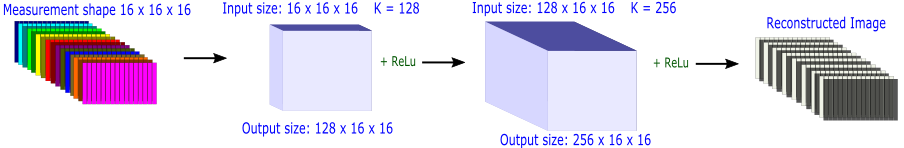
\includegraphics[scale=0.5]{ARCNN1.png} 
\caption[Alpha CNN architecture for recovery ]{Depiction of the alpha CNN architecture.}
\label{fig:ARCNNim1} 
\end{figure}

\subsubsection{Beta CNN network}
During the development of this thesis several attemps for reconstructing images using deep learning were published \cite{kulkarni2016reconnet,mousavi2015deep,iliadis2016deep,iliadis2016deepbinarymask,adler2016deep}. Interestingly, Kulkarni \textit{et al}. \cite{kulkarni2016reconnet} also addressed the problem of CS recovery using a CNN. The other approaches are very similar because they are based on an auto-encoder.  Even more, they do not compressed the images using iid Gaussian matrices. Rather, they learn the sensing matrix $\Phi$ in the first layer. Other interesting findings were made by Kulkarni \textit{et al}. \cite{kulkarni2016reconnet}. They introduced a new parameters that controls the redundancy of the network. Redundancy refers to how large the network will be in relation with the size of the original image. For example, a redundancy factor of 8, would create a reconstruction layer of size $redundancy \times N$. The value 8 turned out to yield better reconstruction performance according to their tests.\\\\
Based on the previous concepts and proved capabilities of the alpha network we proposed another network sketched in Figure \ref{fig:ARCNNim2}. Unlike alpha network, beta network does not receive compressed measurements as input. Rather, the original image interpreted as blocks is reshaped into a 3D tensor. Doing that, allows the network to learn the sensing matrix, in fact the first layer is interpreted as the compression step. The second layer and third layers are called reconstructions layers. The output layer reshapes the data back to the original image size and is the last step in the recovery process.         
\begin{figure}[tb] 
\centering 
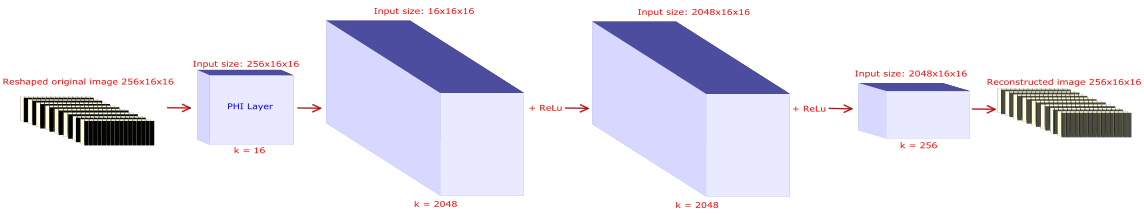
\includegraphics[scale=0.5]{ARCNN2.png} 
\caption[Beta CNN architecture for recovery ]{Depiction of the beta CNN architecture. Notice the first layer is learning the sensing matrix $\Phi$.}
\label{fig:ARCNNim2} 
\end{figure}

\section{Training CNN's}
Training is the process of learning the values of the parameters of the networks. During this step one is concerned with choosing an appropriate weight initialization, loss function, parameter update rule and batch size.

\subsection{Weight initialization}
Choosing the right initial values of the network is needed to secure a sucessful convergence. Furthermore, it can avoid problems like vanishing gradients or ending up being stuck in local minima. Using independent Gaussian random numbers is a very common practice for simple networks but, as complexity increases, smarter ways had been investigated \cite{glorot2010understanding}. Glorot and Bengio empirically validated a method to initialize the weights called normalized initialization 
\begin{equation} \label{eq:Initw1}
\hspace{3em} \hspace{3em} \hspace{3em} W \sim U [ - \frac{\sqrt{6}}{\sqrt{n_j + n_{j+1}}}, \frac{\sqrt{6}}{\sqrt{n_j + n_{j+1}}} ] \enspace \enspace \hspace{3em}
\end{equation}  
were $n_j$ is the layer size of layer $j$. In this thesis we follow the same approach.   

\subsection{Loss function}
Since we need a measure of how good the reconstruction from compressed measurements is, we need to define a way to compare the difference (error) against the original image. Not only that, the loss function also serves as an objective that we would like to minimize as much as possible. The choice of the loss functions depends on the type of problem that one is facing, regression or classification, in order to achieve better results. We have chosen to use the mean square error as the loss function (MSE) because it is highly related to an evaluation metric (PSNR) that we will explain later. The MSE is mathematically defined as 
\begin{equation} \label{eq:MSE1}
\hspace{3em} \hspace{3em} \hspace{3em} L (w) = \frac{1}{N} \sum\limits_{n=1}^N \Vert f(x_n,w) - y_n\Vert_{2}^2 \enspace \enspace \hspace{3em}
\end{equation} 
were $N$ is the number of images in the dataset, $\hat{x} = f(x_n,w)$ represents the nonlinear mapping computed by the CNN and $y_n$ is the original image. Using backpropagation, we train the CNN by minimizing the loss function defined in \ref{eq:MSE1}.  

\subsection{Parameter update rule}     
The easiest way to update the weights $\omega$ is by following the negative direction of the loss function using SGD as we explanied previously \ref{sec:NNs}. As with initialization methods, the algorithms to find a minimum abound. For our training, we use Adam (Adaptive moment estimation) \cite{kingma2014adam} as it converges faster compared to other algorithms. \

It works by storing the weighted decay of the previous square gradient $v_t$ and previous gradient $m_t$. Subsequently, $v_t$ and $m_t$ are corrected in order to eliminate initial bias. Those estimates are used along with SGD as a way to adapt learning rates for parameter $\omega$. The full algorithm  as we use it goes     

\begin{algorithm}
\caption{Adam update}
\label{Adamalg}
\begin{algorithmic}[2]
    \Require $\alpha = 0.0005 $: Stepsize, $\epsilon = 10^{-8}$ 
    \Require $\beta_1 = 0.9$, $\beta_2 = 0.999$: Exponential decay rats for moment estimates
    \Require $L ( \omega ) $: Loss function
    \Require $ \omega_0 $: Initial parameter values
    \State $m_0 \leftarrow 0$ (Initialize $1^{st}$ moment vector)
    \State $v_0 \leftarrow 0$ (Initialize $2^{nd}$ moment vector)
    \State $t \leftarrow 0$ (Initialize timestep)
    \While{$\omega_t$ not converged}
        \State $t \leftarrow t+1$ 
        \State $g_t \leftarrow \nabla_{\omega} L_t ( \omega_{t-1} )$ (Gradient of loss function at time step $t$)
        \State $m_t \leftarrow \beta_1 \cdot m_{t-1} + ( 1 -  \beta_1) \cdot g_t $ (Update biased first moment estimate)
        \State $v_t \leftarrow \beta_2 \cdot v_{t-1} + (1 - \beta_2) \cdot g_{t}^2 $ (Update biased second moment estimate)
        \State $\hat{m}_t \leftarrow \frac{m_t}{( 1 - \beta_{1}^{t} )}$  (Compute bias-corrected first moment estimate)
        \State $\hat{v}_t \leftarrow \frac{m_t}{( 1 - \beta_{2}^{t} )}$  (Compute bias-corrected second moment estimate)
        \State $\omega_t \leftarrow \omega_{t-1} - \alpha \cdot \frac{ \hat{m}_t }{ ( \sqrt{\hat{v}_t } + \epsilon ) } $ (Update parameters)

    \EndWhile
    
    \State \Return $\omega_t $ (Resulting parameters)   
\end{algorithmic}
\end{algorithm}

\subsection{Batch size training}  
For training our CNN's and results presented later we have used a batch size of 20. 


\section{Postprocessing of reconstructed images}
As it can be inferred from Figure \ref{fig:ARCNNim2} that the output of the CNN is not an image. Rather, it is a 3D tensor from which, with minor extra postprocessing, we recover the image. This process aims to invert the prepocessing step explained in section \ref{sec:prepro}. \\\\

First the image is reshaped back to ist original size $N \times N$. Then using col2im MATLAB commnad get the reconstructed image ready to be visualized. Image \ref{fig:Posproim1} shows the procedure. Optionally, we also make use of the very common image denoiser BM3D \cite{dabov2007image}. That is because we would like to get rid of the block nature previously explained. 

\begin{figure}[tb] 
\centering 
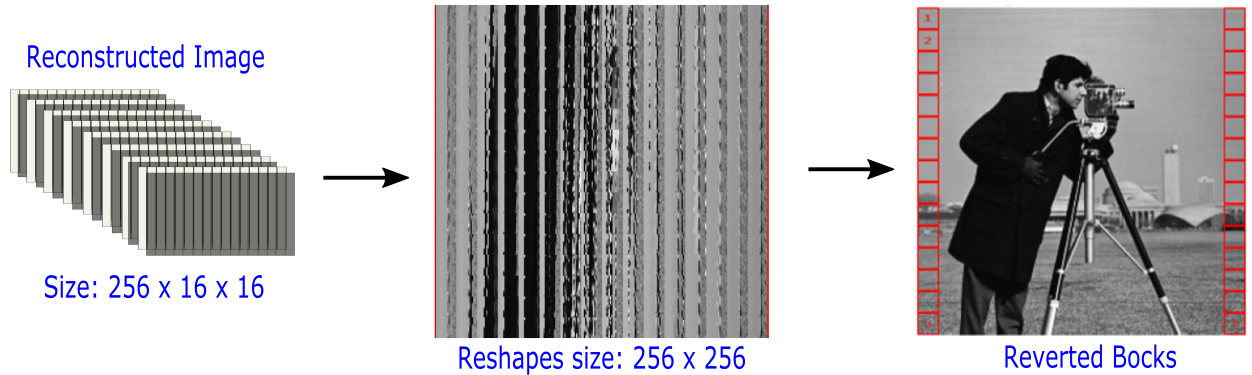
\includegraphics[scale=0.6]{POSPRO1.png} 
\caption[Postprocessing of recovered images ]{Postprocessing illustration to visualize the reconstructed image.}
\label{fig:Posproim1} 
\end{figure}

\section{Evaluation metrics}
Whenever images are undergoing any type of processing, they are bound to suffer a deprecation of the visual quality. Namely, for applications that are ultimately perceived by human eye, there is a need to precisely evaluate the degradation rate (noise) in the image that a certain algorithm adds. Even though agreeing on a metric that is capable of fairly measureing the visual impact is somewhat subjective, there are two methods widely used for that purpose Peak signal-noise-to ratio (PSNR) and Structural similariry index (SSIM) \cite{wang2004image}.     

\subsection{PSNR} 
The most common and straightforward way to compute measurement metric is the mean square error (MSE) \ref{eq:MSE1}. It is obtained by averaging the difference between the original pixel values of an image and the pixel values of a reconstructed image. By using the MSE of the original image $I$ and reconstructed $RI$, the PSNR expressed in decibels (dB) is calculated as
\begin{equation} \label{eq:mse1}
\hspace{3em} \hspace{3em} \hspace{3em} MSE = \frac{1}{NN} \sum\limits_{i=1}^N \sum\limits_{j=1}^N [ I( i , j) - RI ( i , j ) ]^2    \enspace \enspace \hspace{3em}
\end{equation} 

\begin{equation} \label{eq:LS1}
\hspace{3em} \hspace{3em} \hspace{3em} PSNR = 10 \cdot log_{10} \bigg( \frac{ MAX_{I}^{2} }{MSE} \bigg) \enspace \enspace \hspace{3em}
\end{equation} 

Here, $MAX_{I}^{2}$ is the maximum pixel value of the image. For grayscale image such value is $(2^8 - 1)$ when using 8 bits per pixel. PSNR has the advantages of being simple and mathematically suited from the optimization point of view but, it also has two major disadvantages: it fails to capture the effects on the structure of the image which means that two images with the same MSE may have a considerable visual impact difference and it does not consider the human perception system. Desired values for PSNR should be above 30dB. 

\subsection{SSIM}
SSIM is a method measuring the similarity between two images. Unlike PSRN, it uses a more complex approach to computing the difference in accordance with the human visual perception. It takes into consideration three features of an image: luminance ($l$), contrast ($c$) and structure ($s$). For two images $I$ and $RI$, each term is evaluated as
\begin{equation} \label{eq:Lumi}
\hspace{3em} \hspace{3em} \hspace{3em} l(I,RI)= \frac{2\mu_{I} \mu_{RI} + C_1}{\mu_{I}^2 + \mu_{RI}^2 + C_1} \enspace \enspace \hspace{3em}
\end{equation}
\begin{equation} \label{eq:contra}
\hspace{3em} \hspace{3em} \hspace{3em} c(I,RI)= \frac{2\sigma_{I} \sigma_{RI} + C_2}{\sigma_{I}^2 + \sigma_{RI}^2 + C_2} \enspace \enspace \hspace{3em}
\end{equation}
\begin{equation} \label{eq:Struct}
\hspace{3em} \hspace{3em} \hspace{3em} s(I,RI)= \frac{\sigma_{IRI} + C_3}{\sigma_{I} \sigma_{RI} + C_3} \enspace \enspace \hspace{3em}
\end{equation}
variables $\mu_{I}$, $\mu_{RI}$, $\sigma_{I}$, $\sigma_{RI}$ and $\sigma_{IRI}$ represent local means, standard deviations and cross-covariance of images I and RI. Arguments $C_1$, $C_2$ and $C_3$ are predefined constants. The final index is weighted a multiplication of the terms
\begin{equation} \label{eq:ssim1}
\hspace{3em} \hspace{3em} \hspace{3em} SSIM(I,RI)= \big[ l(I,RI)^{\alpha} \cdot c(I,RI)^{\beta} \cdot s(I,RI)^{\gamma} \big]   \enspace \enspace \hspace{3em}
\end{equation}
In practice $\alpha = \beta = \gamma = 1$, and $C_3 = \frac{C_2}{2}$ simplifying to
\begin{equation} \label{eq:ssim2}
\hspace{3em} \hspace{3em} \hspace{3em} SSIM(I,RI)= \frac{(2\mu_{I} \mu_{RI} + C_1)(2\sigma_{IRI}+C_2)}{(\mu_{I}^2 + \mu_{RI}^2 + C_1)(\sigma_{I}^2 \sigma_{RI}^2 + C_2)}   \enspace \enspace \hspace{3em}
\end{equation}
This index can have values ssim $\in [0,1]$ with $0$ meaning that the images are not similar at all and with $1$ meaning that images are exactly the same. Ssim values above 0.7 are considered sufficiently good for any reconstruction algorithm.  

    
 


  
